\section{Theoretical Analysis}
\label{sec:analysis}

We start off by analyzing the circuit at the central frequency, the geometric average between the lower and upper cut-off frequencies. In this case, the input impedance is given by the series of resistor $R_1$ and capacitor $C_1$ and the output impedance by the parallel of resistor $R_2$ and capacitor $C_2$. The gain is given by the quotient between $v_{out}$ and $v_{in}$, which is calculated taking into account the fact that this OP-AMP is a non-inverting amplifier. We get the results:

\begin{center}
\begin{tabular}{|l|r|}
  \hline    
  {\bf Variable} & {\bf Value} \\ \hline
  gain & 8.2787e+01\\\hline gaindB & 3.8359e+01\\\hline Zire & 1.0000e+03\\\hline Ziim & -4.6904e+02\\\hline Zore & 8.1967e+02\\\hline Zoim & -3.8446e+02\\\hline 
\end{tabular}
\end{center}

We then do the same type of analysis, but with a vector of frequencies, which means we calculate the gain for $f \in [10, 10^8] Hz$. We present its magnitude in dB and its phase in degrees.

\begin{figure}[H] \centering
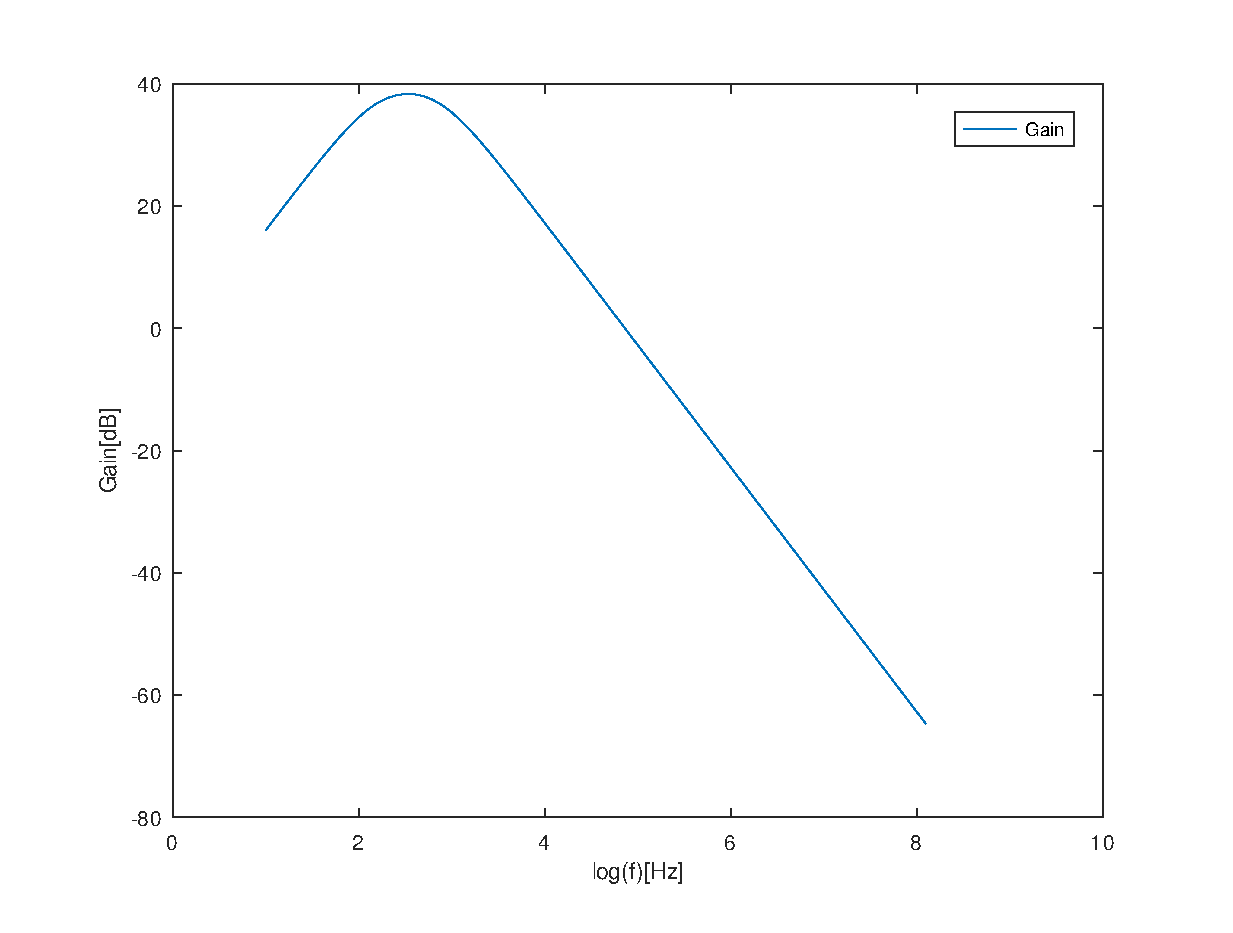
\includegraphics[width=0.5\linewidth]{gainteo.eps}
\caption{Gain in dB}
\label{fig:gainteo}
\end{figure}

\begin{figure}[H] \centering
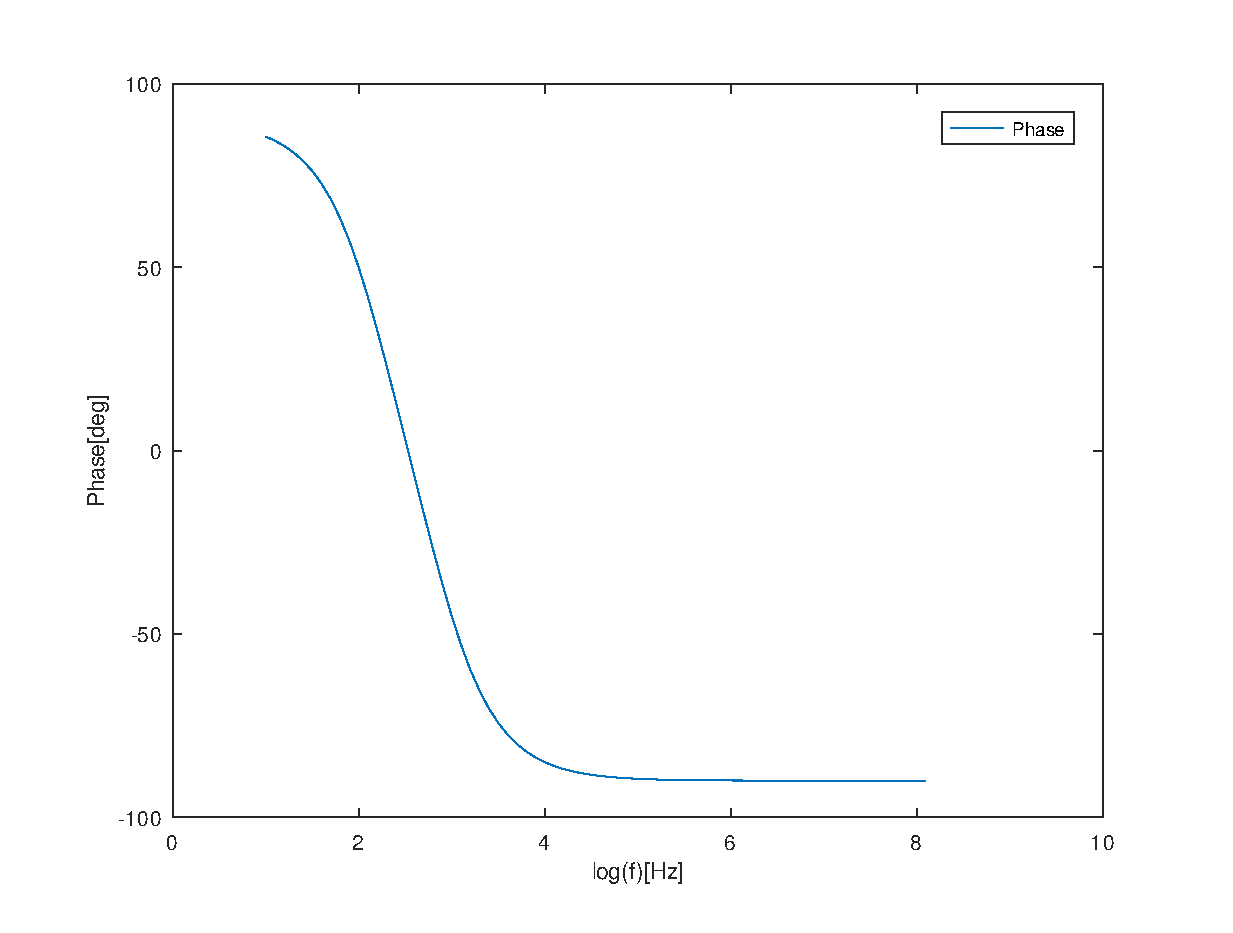
\includegraphics[width=0.5\linewidth]{phaseteo.eps}
\caption{Phase in degrees}
\label{fig:phaseteo}
\end{figure}